\documentclass{article}%
\usepackage[T1]{fontenc}%
\usepackage[utf8]{inputenc}%
\usepackage{lmodern}%
\usepackage{textcomp}%
\usepackage{lastpage}%
\usepackage{authblk}%
\usepackage{graphicx}%
%
\title{Genotyping and Phenotyping of Beta2{-}Toxigenic Clostridium perfringens Fecal Isolates Associated with Gastrointestinal Diseases in Piglets}%
\author{Gary Norman}%
\affil{Blood Transfusion Centre of Slovenia, Ljubljana, Slovenia}%
\date{01{-}01{-}2013}%
%
\begin{document}%
\normalsize%
\maketitle%
\section{Abstract}%
\label{sec:Abstract}%
Each year, cancer researchers discover new ways to control cancer growth in cells while avoiding its recurrence. Perhaps an even more powerful method would be the discovery of a chemical called c{-}secretase inhibitor, the monoclonal antibody antibody dubbed "RITE" in earlier days, that decreases cancer cell growth by signaling the uptake of nutrients, enabling the cancer to survive.\newline%
Most chemotherapies use radiation to target a specific chemical. Ineffectively, these agents destroy cancer cells but kill most healthy cells as well. Such agents are generally chemically reversible: the goal is to prevent the unwanted growth, but for some reason the tumors mutate the chemical, thus breaking off from the protein{-}targeting organ. C{-}secretase inhibitor had been caught and battled with this dilemma.\newline%
Meanwhile, c{-}secretase inhibitor's key chemical, the proteasome, seems to not only block the synthesis of the cancer drug but inhibits the macrophage (specifically the RCC), preventing the organ from performing any function. By inhibiting C{-}secretase inhibitor production in normal cancer cells, the C{-}secretase inhibitor is then able to protect normal tissue and differentiate and divide, providing a universal target.\newline%
Disruption of expression of a gene that is expressed in the bodys innate immune system, BRAF1, on a tumor{-}stimulating surface receptor in lymphocytes, could be the answer.\newline%
In early research, c{-}secretase inhibitor has already been found to have some of the same features as an EGFR inhibitor or a proteasome inhibitor like emicizumab, which produces similar effects.\newline%
Funding for the study was provided by Organogenesis, Inc., California Genomics Institute and Centre for NanoArray Interventions.

%
\subsection{Image Analysis}%
\label{subsec:ImageAnalysis}%


\begin{figure}[h!]%
\centering%
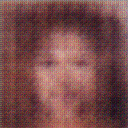
\includegraphics[width=150px]{500_fake_images/samples_5_394.png}%
\caption{A Man In A Suit And Tie Is Smiling}%
\end{figure}

%
\end{document}